% Uncomment this to make slides with overlays:
%\documentclass[slides]{beamer}

% Uncomment these (but comment the above \documentclass line) to make handouts:
\documentclass[handout]{beamer}

% Uncomment these to have more than one slide per page
\usepackage{pgfpages}
\pgfpagesuselayout{2 on 1}[border shrink=5mm]
\pgfpageslogicalpageoptions{1}{border code=\pgfusepath{stroke}}
\pgfpageslogicalpageoptions{2}{border code=\pgfusepath{stroke}}

\usepackage[]{graphicx, color, hyperref}

\mode<presentation>
{
	%\usetheme[secheader]{Boadilla}
	%\usecolortheme[rgb={.835, .102,.169}]{structure}  
	\usetheme[width= 0cm]{Goettingen}
	%\setbeamercovered{transparent}
}
\setbeamertemplate{navigation symbols}{}
\setbeamertemplate{footline}[frame number]

\definecolor{blue2}{rgb}{0.278,0.278,0.729} 
\newcommand{\blue}[1]{\textcolor{blue2}{#1}}
\newcommand{\white}[1]{\textcolor{white}{#1}}
\newcommand{\red}[1]{\textcolor{red}{#1}}
\newcommand{\xbar}{\overline{x}}
\newcommand{\ybar}{\overline{y}}
\newcommand{\phat}{\widehat{p}}
\newcommand{\prob}{\mbox{Pr}}
\newcommand{\E}{\mathbb{E}}
\newcommand{\Var}{\mbox{Var}}
\newcommand{\cp}{\oplus}
\newcommand{\cm}{\circleddash}


\title{Lecture 22: Chi-Square Tests for Goodness-of-Fit}
\author{Chapter 6.3}
\date{}


\begin{document}
%------------------------------------------------------------------------------
\begin{frame}
\titlepage
\end{frame}
%------------------------------------------------------------------------------


%------------------------------------------------------------------------------
\begin{frame}[fragile]
\frametitle{Question for Today}
Say we have a population where the racial breakdown of the juror pool (registered voters) is:

\begin{center}
\begin{tabular}{l||cccc|c}
Race & White & Black & Hispanic & Other & Total \\ 
\hline
Registered Voters & 72\% & 7\% & 12\% & 9\% & 100\%\\ 
\textcolor{white}{Representation} & \textcolor{white}{0} & \textcolor{white}{0} & \textcolor{white}{0} & \textcolor{white}{100} & \textcolor{white}{$n=100$} \\ 
\end{tabular}
\end{center}

\end{frame}
%------------------------------------------------------------------------------


%------------------------------------------------------------------------------
\begin{frame}[fragile]
\frametitle{Question for Today}
Say we had $n=100$ people picked as jurors, we \blue{expect} the breakdown to be:

\begin{center}
\begin{tabular}{l||cccc|c}
Race & White & Black & Hispanic & Other & Total \\ 
\hline
Registered Voters & 72\% & 7\% & 12\% & 9\% & 100\%\\ 
Representation & 72 & 7 & 12 & 9 & $n=100$ \\ 
\end{tabular}
\end{center}

\end{frame}
%------------------------------------------------------------------------------


%------------------------------------------------------------------------------
\begin{frame}[fragile]
\frametitle{Question for Today}
Say we \blue{observe} the following breakdown.  Fairly obvious bias in juror selection!

\begin{center}
\begin{tabular}{l||cccc|c}
Race & White & Black & Hispanic & Other & Total \\ 
\hline
Registered Voters & 72\% & 7\% & 12\% & 9\% & 100\%\\ 
Representation & 0 & 0 & 100 & 0 & $n=100$ \\ 
\end{tabular}
\end{center}

\end{frame}
%------------------------------------------------------------------------------


%------------------------------------------------------------------------------
\begin{frame}[fragile]
\frametitle{Question for Today}

But what about the following?  We expected 72 whites, but observe 75.  Is there a bias?  i.e. a non-random mechanism?

\begin{center}
\begin{tabular}{l||cccc|c}
Race & White & Black & Hispanic & Other & Total \\ 
\hline
Registered Voters & 72\% & 7\% & 12\% & 9\% & 100\%\\ 
Representation & 75 & 6 & 11 & 8 & $n=100$ \\ 
\end{tabular}
\end{center}

\end{frame}
%------------------------------------------------------------------------------


%------------------------------------------------------------------------------
\begin{frame}[fragile]
\frametitle{Chi-Square Tests}

\blue{Chi-square $\chi^2$ tests} allow us to compare
\begin{itemize}
\item Expected frequencies
\item Observed frequencies
\end{itemize}

\vspace{0.5cm}

\pause i.e. What is the \blue{``goodness''} of the fit of the observed counts to the expected counts?



\end{frame}
%------------------------------------------------------------------------------


%------------------------------------------------------------------------------
\begin{frame}[fragile]
\frametitle{The Data}

Let's use $n=275$ people.  Assuming the same proportions as earlier to compute the \blue{expected} counts, say we then observe:

\begin{center}
\begin{tabular}{l||cccc|c}
Race & White & Black & Hispanic & Other & Total \\ 
\hline
Expected Counts & 198 & 19.25 & 33 & 24.75 & 275\\ 
\pause Observed Counts & 205 & 26 & 25 & 19 & 275\\ 
\end{tabular}
\end{center}

\end{frame}
%------------------------------------------------------------------------------


%------------------------------------------------------------------------------
\begin{frame}[fragile]
\frametitle{Hypothesis Test}
\begin{eqnarray*}
H_0:&& \mbox{\blue{the jurors are a random sample}}\\
&& \mbox{i.e. there is no racial bias in who serves on a jury and}\\
&& \mbox{the observed counts reflect natural sampling fluctuation}\\
\mbox{vs } H_A:&& \mbox{\blue{the jurors are not randomly sampled}}\\
&& \mbox{i.e. there is racial bias in juror selection}
\end{eqnarray*}
\end{frame}
%------------------------------------------------------------------------------


%------------------------------------------------------------------------------
\begin{frame}[fragile]
\frametitle{Hypothesis Test:  }

We compute a \blue{test statistic} and use a \blue{null distribution} (the distribution of the test statistic if $H_0$ is true) to compute p-values:

\begin{enumerate}
\pause\item \blue{means/proportions}:
\begin{itemize}
\item test statistic: $z$-score of $\xbar / \widehat{p}$
\item null distribution: normal distribution ($z$-table)
\end{itemize}
\pause\item \blue{t-test}:  
\begin{itemize}
\item test statistic: $t$-statistic
\item null distribution: t-distribution with $df=n-1$ ($t$-table)
\end{itemize}
\pause\item \blue{AVOVA}:  
\begin{itemize}
\item test statistic: $F$-statistic 
\item null distribution: $F$-distribution with $df_1=k-1$ and $df_2 = n-k$ ($F$-table)
\end{itemize}
\pause\item Now: \blue{Goodness-of-fit}:
\begin{itemize}
\item test statistic: $\chi^2$-statistic
\item null distribution: $\chi^2$ distribution with $df=k-1$
\end{itemize}
\end{enumerate}

\end{frame}
%------------------------------------------------------------------------------


%------------------------------------------------------------------------------
\begin{frame}[fragile]
\frametitle{Test Statistic}

For previous tests, we constructed a test statistic of the following form:  
\[
\frac{\mbox{point estimate} - \mbox{null value}}{\mbox{SE of point estimate}}
\]
\pause In our case, it's similar.  For each of the $k$ groups (in this case racial group) compute
\[
Z = \frac{\mbox{observed count} - \mbox{expected count}}{\sqrt{\mbox{expected count}}}
\]
\end{frame}
%------------------------------------------------------------------------------


%------------------------------------------------------------------------------
\begin{frame}[fragile]
\frametitle{Test Statistic}
\[
Z = \frac{\mbox{observed count} - \mbox{expected count}}{\sqrt{\mbox{expected count}}}
\]

So when 
\begin{itemize}
\item observed = expected $\Rightarrow$ $Z=0$
\item observed $>$ expected $\Rightarrow$ $Z>0$
\item observed $<$ expected $\Rightarrow$ $Z<0$
\end{itemize}

\end{frame}
%------------------------------------------------------------------------------


%------------------------------------------------------------------------------
\begin{frame}[fragile]
\frametitle{Test Statistic}
Now treat $+$'ve and $-$'ve differences as the same:
\begin{eqnarray*}
Z^2 &=& \left(\frac{\mbox{observed count} - \mbox{expected count}}{\sqrt{\mbox{expected count}}}\right)^2\\
&=& \frac{(\mbox{observed count} - \mbox{expected count})^2}{\mbox{expected count}}
\end{eqnarray*}

\pause Why square it and not absolute value it?  It's easier to do \blue{calculus} on $x^2$ than $|x|$.
\end{frame}
%------------------------------------------------------------------------------


%------------------------------------------------------------------------------
\begin{frame}[fragile]
\frametitle{Test Statistic}
In the case of our trial data, we have 4 groups: white, black, hispanic, and other:
\begin{eqnarray*}
\chi^2 &=& Z_w^2 + Z_b^2 + Z_h^2 + Z_o^2\\
&=& \frac{(205-198)^2}{198} + \frac{(26-19.25)^2}{19.25} + \frac{(25-33)^2}{33} + \frac{(19-24.75)^2}{24.75}\\
&=& 5.89
\end{eqnarray*}

\pause \blue{This is our test statistic}.
\end{frame}
%------------------------------------------------------------------------------


%------------------------------------------------------------------------------
\begin{frame}[fragile]
\frametitle{p-values}
To compute the p-value, we compare the test statistic to a $\chi^2$ distribution with $df=k-1$ degrees of freedom.  Note: not $df=n-1$ like with t-test.  

\vspace{0.25cm}

\begin{center}
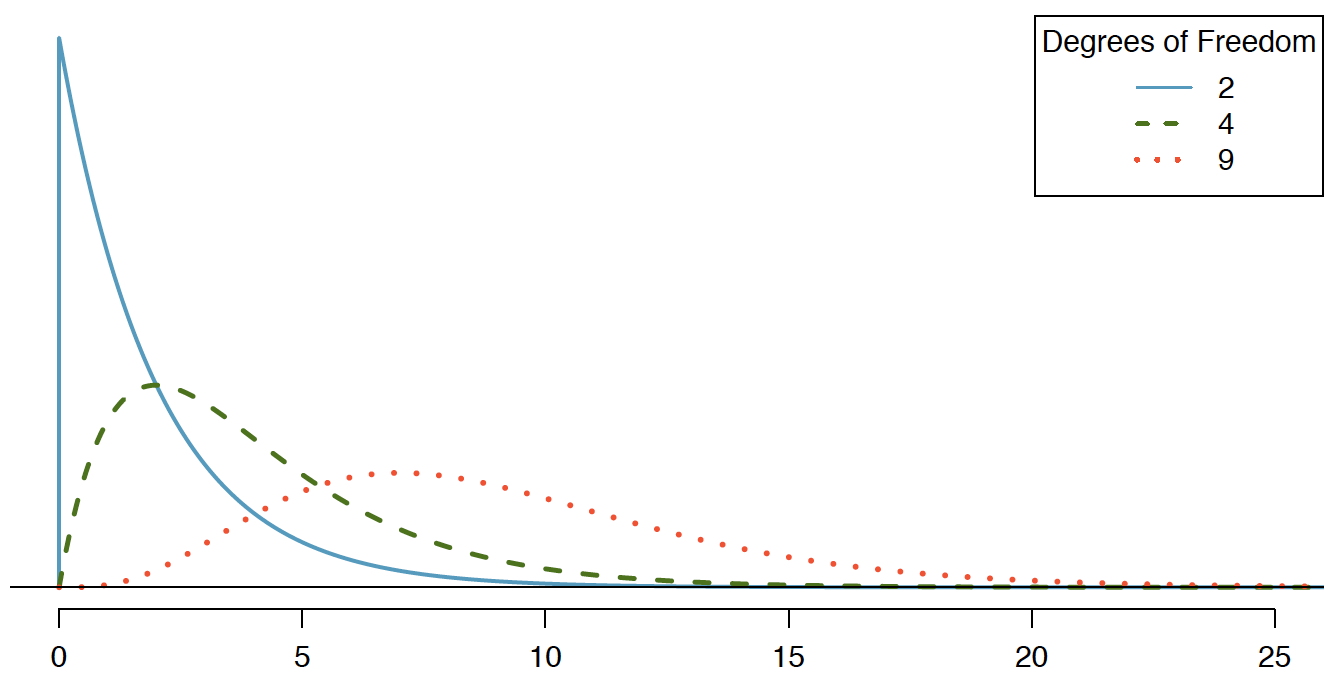
\includegraphics[width=0.8\textwidth]{figure/chi.png}
\end{center}

\end{frame}
%------------------------------------------------------------------------------


%------------------------------------------------------------------------------
\begin{frame}[fragile]
\frametitle{p-value}
Use table on page 412:
\begin{center}
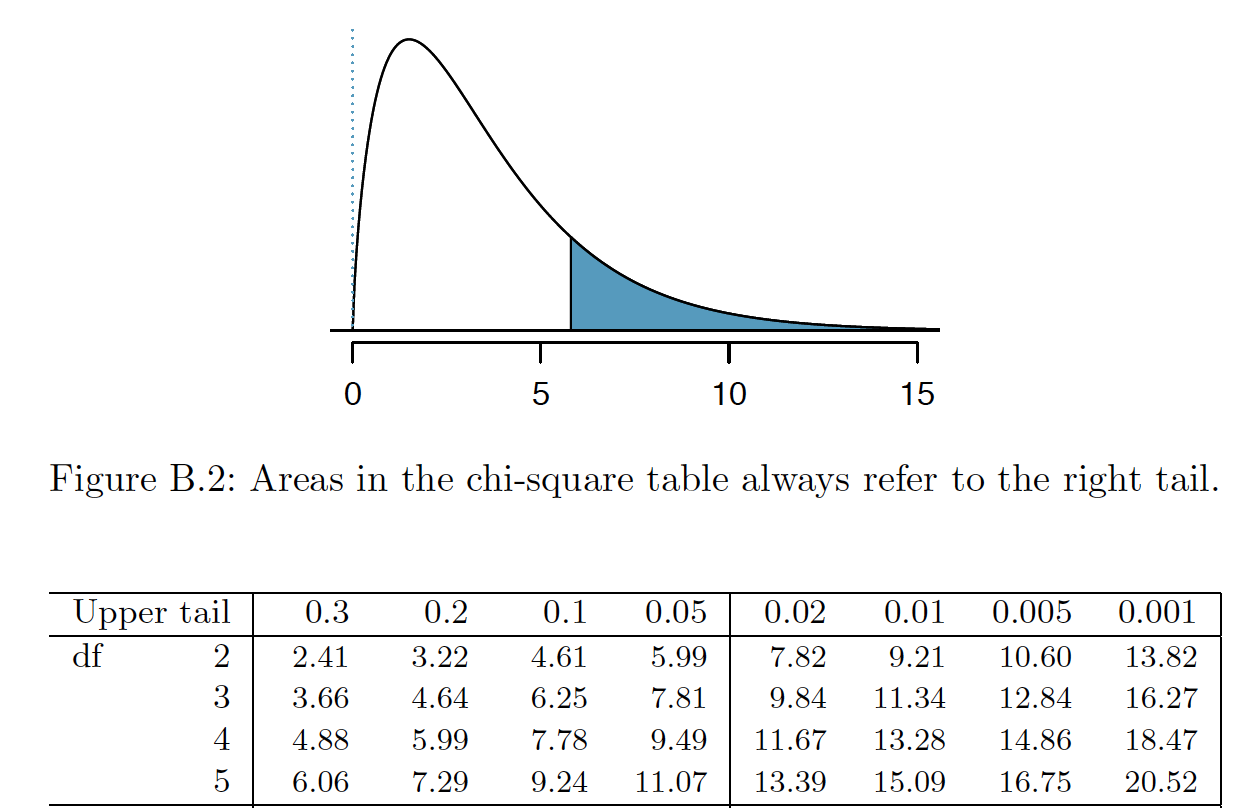
\includegraphics[width=0.8\textwidth]{figure/table.png}
\end{center}
\pause In our case, $df=k-1=3$, and $\chi^2=5.89$, which is in between $(4.64, 6.25)$, so p-value is in between $(0.1, 0.2)$.  Not overwhelming evidence against $H_0$.  

\end{frame}
%------------------------------------------------------------------------------


%(0-198)^2/sqrt(198) + (0-19.25)^2/sqrt(19.25) + (0-33)^2/sqrt(33) + (275-24.75)^2/sqrt(24.75)
%------------------------------------------------------------------------------
\begin{frame}[fragile]
\frametitle{Hypothetical Scenarios}
\begin{center}
\begin{tabular}{l||cccc|c}
Race & White & Black & Hispanic & Other & Total \\ 
\hline
Expected Counts & 198 & 19.25 & 33 & 24.75 & 275\\ 
Observed Counts &  &  &  &  & 275 \\ 
\end{tabular}
\end{center}

\pause Say:
\begin{itemize}
\item For all 4 groups, we observed = expected.  Then
\[
Z_i^2=\frac{(\mbox{observed count}_i - \mbox{expected count}_i)^2}{\mbox{expected count}_i} = 0
\]
for $i=1,\ldots,4$, and $\chi^2=0$.  p-value = 1
\pause\item Say we observed 0 whites, blacks, hispanics and 275 others, then $\chi^2=15648.25$.  p-value=0
\end{itemize}

\end{frame}
%------------------------------------------------------------------------------


%------------------------------------------------------------------------------
\begin{frame}[fragile]
\frametitle{Chi-Square Test for One-Way Tables}
This is also called a \blue{chi-square test for one-way tables}.  

\begin{eqnarray*}
\chi^2 &=& \sum_{i=1}^k Z_i^2 = \sum_{i=1}^k \frac{(\mbox{observed count}_i - \mbox{expected count}_i)^2}{\mbox{expected count}_i}\\
%&=& \frac{(\mbox{observed count}_1 - \mbox{expected count}_1)^2}{\mbox{expected count}_1} + \ldots +\\
%&& \frac{(\mbox{observed count}_k - \mbox{expected count}_k)^2}{\mbox{expected count}_k}
\end{eqnarray*}

\end{frame}
%------------------------------------------------------------------------------


%------------------------------------------------------------------------------
\begin{frame}[fragile]
\frametitle{Assumptions for Chi-Square Test}
\begin{enumerate}
\pause \item \blue{Independence}:  Each case is independent of the other
\pause\item \blue{Sample size/distribution}:  Similarly like with proportions, we need at least 5 cases in each scenario (each cell in the table)
\pause\item \blue{Degrees of freedom}:  We need at least $df=2$, i.e. $k\geq 3$
\end{enumerate}

\end{frame}
%------------------------------------------------------------------------------


%------------------------------------------------------------------------------
\begin{frame}[fragile]
\frametitle{Next Time}
We look at \blue{chi-square tests for two-way tables} to test for \blue{independence}.  i.e. are two variables independent from each other?

\end{frame}
%------------------------------------------------------------------------------


\end{document}










